% !TeX program = xelatex
\documentclass[UTF8,12pt,a4paper,fontset=windows]{ctexart}

\usepackage[a4paper,top=23mm,bottom=23mm,left=24mm,right=24mm,headheight=16pt]{geometry}
\usepackage{amsmath,amssymb,mathtools,bm}
\usepackage{graphicx}
\usepackage{booktabs,longtable,tabularx,array,multirow}
\usepackage{siunitx}
\usepackage{xcolor}
\usepackage[most]{tcolorbox}
\usepackage{enumitem}
\usepackage{fancyhdr}
\usepackage{hyperref}
\usepackage{caption}
\usepackage{subcaption}
\usepackage{pgfplots}
\usepackage{tikz}
\usepackage{float}
\usepackage{microtype}

\pgfplotsset{compat=1.18}
\graphicspath{{figures/}}
\sisetup{detect-all,group-separator={,},group-minimum-digits=4,group-digits=integer}

\definecolor{navy}{HTML}{172B4D}
\definecolor{blue}{HTML}{2E74B5}
\definecolor{lightblue}{HTML}{E8F1F8}
\definecolor{lightgray}{HTML}{F2F4F7}
\definecolor{gold}{HTML}{8A6500}
\definecolor{green}{HTML}{287D3C}
\definecolor{red}{HTML}{9B1C1C}

\hypersetup{
  unicode=true,
  pdfencoding=auto,
  colorlinks=true,
  linkcolor=blue,
  citecolor=blue,
  urlcolor=blue,
  pdftitle={基于 CarSim 的半车道路预瞄 QP-MPC 联合仿真技术报告},
  pdfauthor={悬架控制项目组}
}

\pagestyle{fancy}
\fancyhf{}
\fancyhead[L]{\small\color{navy}CarSim 主动悬架联合仿真}
\fancyhead[R]{\small\color{navy}QP-MPC 技术报告}
\fancyfoot[C]{\small\color{gray}\thepage}
\renewcommand{\headrulewidth}{0.4pt}
\renewcommand{\footrulewidth}{0pt}

\ctexset{
  section={format=\Large\bfseries\color{blue},beforeskip=18pt,afterskip=9pt},
  subsection={format=\large\bfseries\color{blue},beforeskip=14pt,afterskip=7pt},
  subsubsection={format=\normalsize\bfseries\color{navy},beforeskip=10pt,afterskip=5pt}
}

\captionsetup{font=small,labelfont=bf,labelsep=quad}
\setlength{\parindent}{2em}
\setlength{\parskip}{2pt}
\setlist[itemize]{leftmargin=2.2em,itemsep=3pt,topsep=4pt}
\setlist[enumerate]{leftmargin=2.5em,itemsep=4pt,topsep=4pt}
\renewcommand{\arraystretch}{1.25}

\newtcolorbox{keybox}[1]{
  enhanced,
  breakable,
  colback=lightblue,
  colframe=blue,
  boxrule=0.7pt,
  arc=1.2mm,
  left=3mm,right=3mm,top=2mm,bottom=2mm,
  title={#1},
  fonttitle=\bfseries\color{blue},
  coltitle=blue
}

\newtcolorbox{notebox}[1]{
  enhanced,
  breakable,
  colback=lightgray,
  colframe=gray!55,
  boxrule=0.5pt,
  arc=1.2mm,
  left=3mm,right=3mm,top=2mm,bottom=2mm,
  title={#1},
  fonttitle=\bfseries\color{navy},
  coltitle=navy
}

\newcolumntype{Y}{>{\raggedright\arraybackslash}X}
\newcommand{\vect}[1]{\bm{#1}}
\newcommand{\trans}{^{\mathsf T}}
\newcommand{\norm}[1]{\left\lVert #1\right\rVert}
\newcommand{\sat}{\operatorname{sat}}
\newcommand{\diag}{\operatorname{diag}}

\begin{document}

\begin{titlepage}
  \centering
  \vspace*{18mm}
  {\small\bfseries\color{blue}阶段汇报 / CarSim--Simulink 联合仿真\par}
  \vspace{11mm}
  {\fontsize{25}{34}\selectfont\bfseries\color{navy}
    基于 CarSim 的半车道路预瞄\\[2mm]
    QP-MPC 联合仿真\par}
  \vspace{8mm}
  {\Large\color{gray}实现说明与多路面联合仿真结果\par}
  \vspace{16mm}
  \begin{tcolorbox}[width=0.88\textwidth,colback=lightblue,colframe=blue,boxrule=0.8pt,arc=1.5mm]
    \begin{tabularx}{\linewidth}{>{\bfseries\color{navy}}p{28mm}X}
      方案定位 & 闭环联调验证：半车 QP-MPC + CarSim 高保真整车\\
      仿真平台 & CarSim 2020 / MATLAB R2026a / Simulink\\
      控制对象 & 前、后轴作动力；左右轮等分，不主动控制侧倾\\
      控制周期 & \SI{0.01}{s}，预测域 \SI{0.20}{s}\\
      结果数据 & 2026 年 8 月 18 日联合仿真\\
      报告整理 & 2026 年 8 月 18 日
    \end{tabularx}
  \end{tcolorbox}
  \vfill
  {\large\bfseries\color{navy}悬架控制项目组\par}
  \vspace{7mm}
\end{titlepage}

\pagenumbering{Roman}
\begin{abstract}
本报告记录半车道路预瞄 QP-MPC 与 CarSim 整车模型的联合仿真实现及验证结果。控制器采用四自由度半车线性模型，每 \SI{10}{ms} 求解一次有限时域凸二次规划，优化前、后轴作动力。道路输入采用固定空间分辨率和感知距离的传感器模型，再由实时车速映射到预测时域；预瞄误差则通过固定空间噪声、偏置和行程约束收紧进行考察。CarSim 内部积分步长与 Simulink 外部步长统一为 \SI{1}{ms}。在 \SI{35}{km/h} 的坑包、B 级和 C 级道路实验中，车身垂向加速度 RMS 分别降低 \SI{15.29}{\percent}、\SI{32.87}{\percent} 和 \SI{25.13}{\percent}，俯仰角加速度 RMS 分别降低 \SI{13.43}{\percent}、\SI{40.90}{\percent} 和 \SI{31.12}{\percent}。进一步按相同的 \SI{10}{m}--\SI{110}{m} 道路区间完成 \SI{35}{km/h}、\SI{60}{km/h} 和 \SI{80}{km/h} 对照，九组工况的车身和俯仰角加速度 RMS 均低于被动基线，改善率分别为 \SI{15.29}{\percent}--\SI{38.14}{\percent} 和 \SI{6.59}{\percent}--\SI{41.22}{\percent}。固定 \SI{3}{m} 感知范围在 \SI{60}{km/h} 和 \SI{80}{km/h} 时只能覆盖约 \SI{89.8}{\percent} 和 \SI{67.4}{\percent} 的预测域，且高速坑包工况的悬架行程有所增加。结果说明理想主动力版本已经形成有效闭环，但当前标定偏向舒适性；将其直接映射到五档 CDC 阻尼后也未获得 RMS 改善，半主动控制仍需重新建模和标定。

\textbf{关键词：}主动悬架；道路预瞄；模型预测控制；二次规划；CarSim；Simulink
\end{abstract}

\clearpage
{\footnotesize\tableofcontents}
\clearpage
\pagenumbering{arabic}

\section{本阶段工作与结论边界}

本阶段的目标是打通“道路空间预瞄--在线 QP--Simulink--CarSim 整车--结果评估”链路。CarSim 计算整车与道路响应，控制器用四自由度半车模型预测升沉和俯仰运动，并在每个控制周期优化前、后轴作动力。基线采用固定阻尼系数的线性被动悬架，MPC 只在该被动力上叠加残差控制量。

\begin{keybox}{阶段完成情况}
控制器已经显式构造预测矩阵、二次型性能指标以及轴力和轴力变化率约束，并在每个控制周期调用 ADMM 求解器，具备有限时域 QP-MPC 的关键环节。当前预测模型仍是半车模型，同一车轴左右车轮获得相同控制增量，因此没有侧倾控制能力。
\end{keybox}

本次汇报不覆盖以下问题：
\begin{itemize}
  \item 只优化升沉和俯仰方向，未将车身侧倾自由度纳入预测模型；
  \item 左右轮道路输入在状态重构中按前后轴聚合，不适合显著左右不对称路面；
  \item 当前数据只覆盖一个车辆和三个离散车速；每个车速--道路组合均为单次运行，预瞄误差试验也只有固定随机种子，尚不足以形成统计性性能结论；
  \item 悬架行程采用硬约束，但尚未加入松弛变量；遇到不可达状态时，仍可能出现小幅数值超限；
  \item 控制器按 \SI{10}{ms} 周期调度，但尚未记录单次 QP 的平均和最坏求解时间，不能据此判断硬实时能力。
\end{itemize}

\section{CarSim--Simulink 联合仿真架构}

\begin{figure}[H]
  \centering
  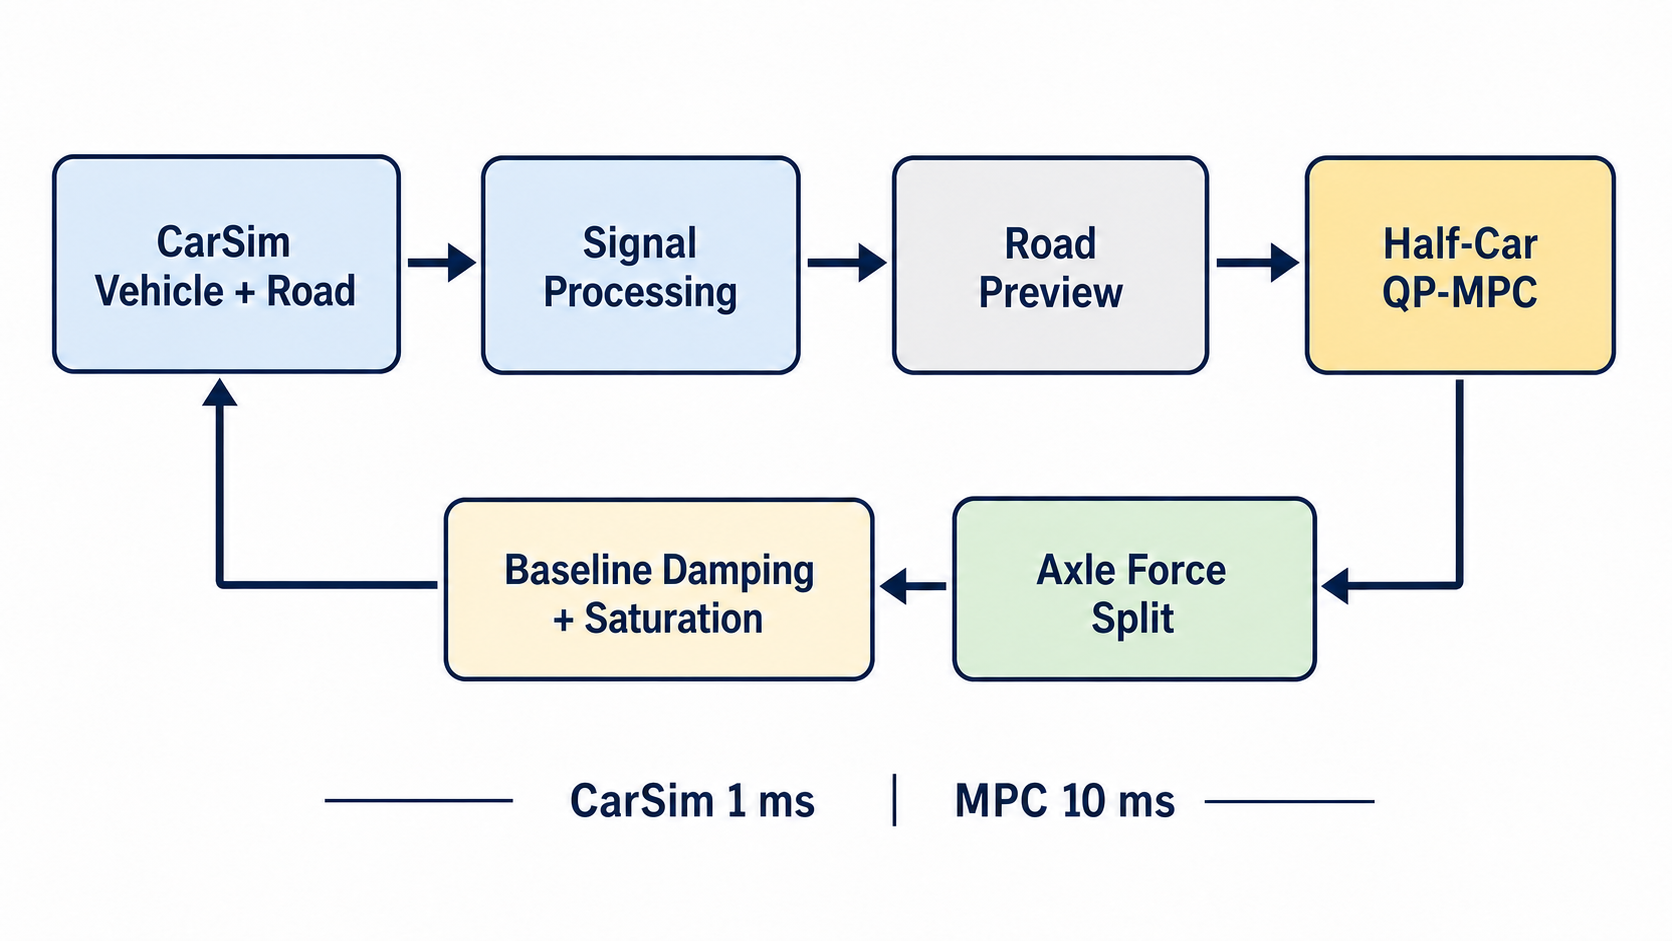
\includegraphics[width=0.98\linewidth]{carsim_mpc_architecture.png}
  \caption{CarSim--Simulink--QP-MPC 联合仿真闭环。模块关系、数据流向和采样周期均按当前工程实现标注。}
  \label{fig:architecture}
\end{figure}

如图~\ref{fig:architecture} 所示，CarSim 输出车身、轮端和车辆定位信号；Simulink 完成单位换算与半车状态重构，其中 CarSim 俯仰量乘以 $-1$ 后转换到车头上仰为正的模型坐标；道路预瞄模块根据轮端当前位置、车辆纵向速度和 CarSim 的 \texttt{ROAD\_DZ} 空间表生成未来 $N=20$ 步道路输入；QP-MPC 输出前、后轴作动力；力分配模块将轴力左右等分并与线性被动阻尼力叠加，最后经角点力饱和后返回 CarSim。

\subsection{Simulink 顶层仿真模型}

\begin{figure}[H]
  \centering
  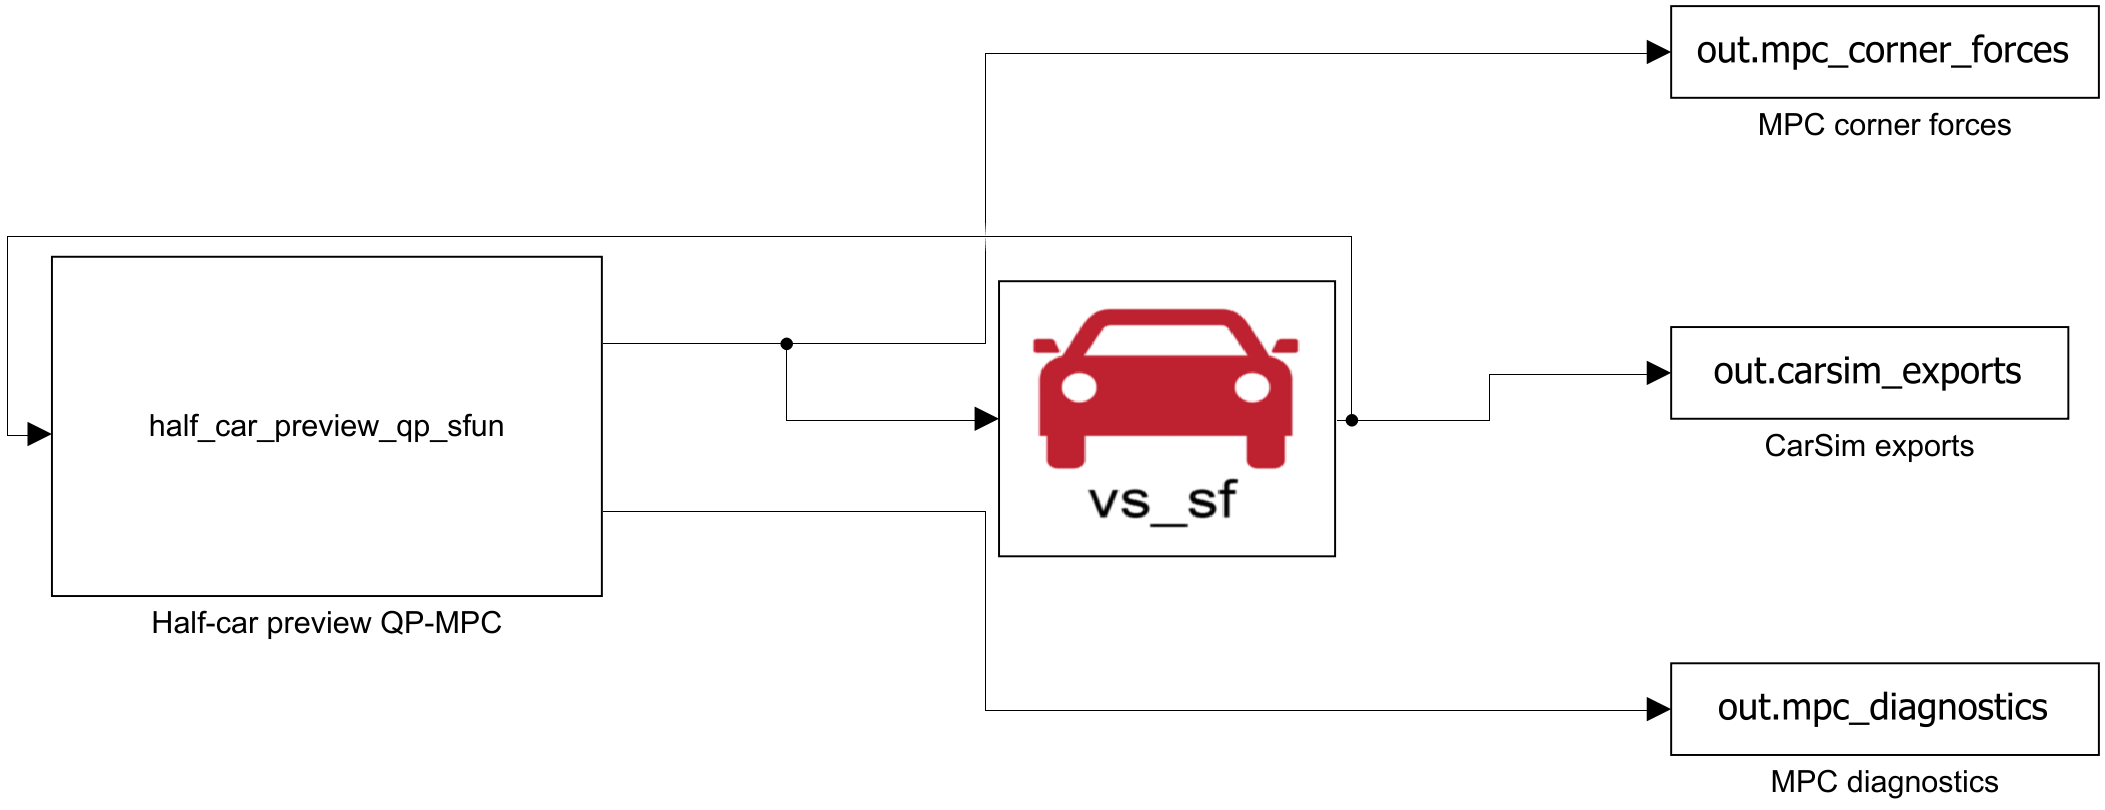
\includegraphics[width=0.99\linewidth]{simulink_carsim_qp_mpc_model.png}
  \caption{实际 \texttt{carsim\_half\_car\_qp\_mpc.slx} 顶层模型。左侧 Level-2 MATLAB S-Function 实现半车预瞄 QP-MPC，中部 CarSim S-Function 执行高保真整车计算，右侧记录角点悬架力、CarSim 导出量和 MPC 诊断量。}
  \label{fig:simulink_model}
\end{figure}

如图~\ref{fig:simulink_model} 所示，CarSim 导出总线进入控制器完成状态重构、道路预瞄和在线 QP 求解；控制器第一输出端返回四角悬架力，第二输出端给出求解器收敛状态、预瞄覆盖率和鲁棒收紧量等诊断。模型采用固定步长离散求解，CarSim 以 \SI{1}{ms} 积分，控制器内部每 \SI{10}{ms} 更新一次控制量。打开该模型前应将 CarSim 的 \texttt{Solver\_SF.slx} 所在目录加入 MATLAB 路径，以保证库链接正常解析。
\subsection{采样与运行参数}

\begin{table}[H]
\centering
\caption{联合仿真主要时间参数}
\begin{tabularx}{0.86\linewidth}{l c X}
\toprule
参数 & 当前值 & 说明\\
\midrule
CarSim 积分步长 & \SI{0.001}{s} & 每个 MPC 周期包含 10 个整车积分步\\
MPC 控制周期 $T_s$ & \SI{0.01}{s} & 控制器每 \SI{10}{ms} 更新一次\\
预测步数 $N$ & 20 & 总预瞄时间为 \SI{0.20}{s}\\
仿真时长 & 按工况设置 & \SI{35}{km/h} 多路面对照为 \SI{12}{s}；车速实验按前轮 \SI{10}{m}--\SI{110}{m} 道路区间统计\\
\bottomrule
\end{tabularx}
\end{table}

CarSim 的运行参数文件还包含内部变量 \texttt{tstep}。仅修改 simfile 中的 \texttt{EXT\_MODEL\_STEP} 会造成 CarSim 物理时间与 Simulink 时间不同步，因此运行脚本会复制一份本地参数文件，并把两处步长同时写为 \SI{1}{ms}。同步后的 \SI{2}{ms} 设置曾在短时试验中引起非线性车辆模型发散，故未采用。\SI{1}{ms} 与原 \SI{0.5}{ms} 结果接近，同时把整车积分次数减半。

\subsection{CarSim I/O 兼容处理}

当前 \texttt{Run\_all.par} 同时启用了 I/O 数据集和 Additional Data 命令，导致四个导入力重复为 8 路、39 个导出量重复为 77 路。适配器向两组导入口发送相同四角力，并读取第 39--77 路的第二组完整输出。若后续在 CarSim GUI 中清除重复配置，应同步修改本地 simfile、S-Function 端口宽度和联合仿真运行脚本。

\section{四自由度半车主动悬架模型}

\begin{figure}[H]
  \centering
  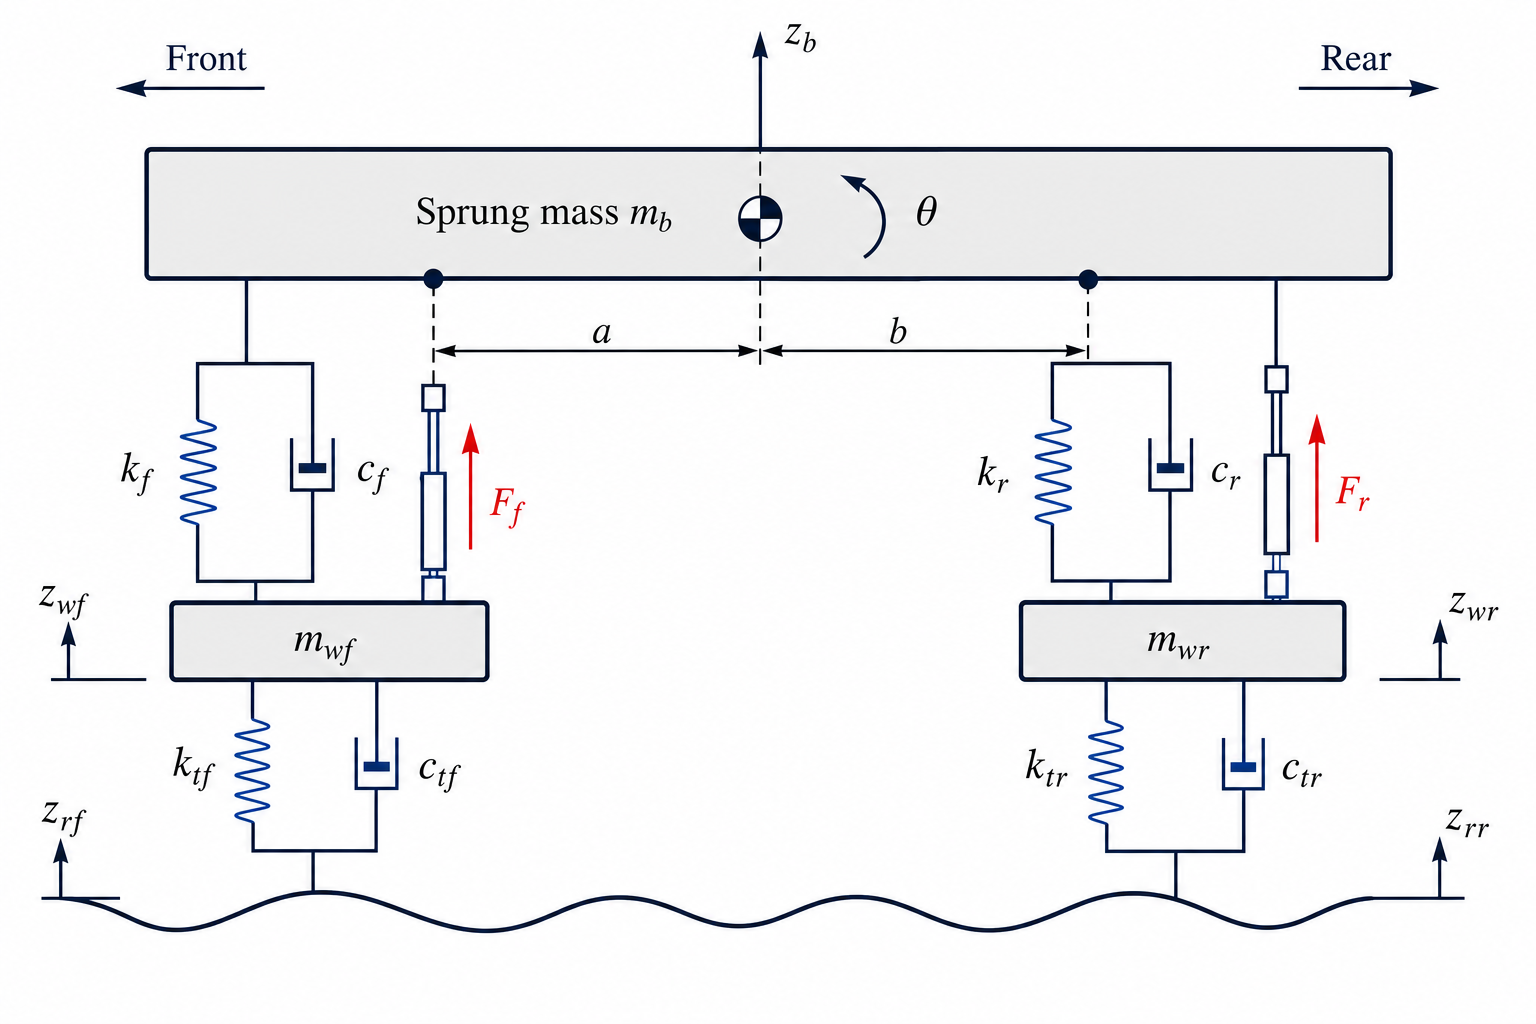
\includegraphics[width=0.98\linewidth]{half_car_active_suspension.png}
  \caption{四自由度半车主动悬架结构。动力学符号、作动力方向和道路输入与当前预测模型一致。}
  \label{fig:halfcar}
\end{figure}

图~\ref{fig:halfcar} 中，$z_b$ 为簧载质量升沉位移，$\theta$ 为俯仰角，$z_{wf}$、$z_{wr}$ 为前后簧下质量位移，$z_{rf}$、$z_{rr}$ 为前后道路输入，$F_f$、$F_r$ 为 MPC 优化的前后轴作动力。$a$、$b$ 分别为车身质心至前、后轴的距离。

\subsection{状态、控制量与道路扰动}

定义状态向量、控制向量和道路扰动为
\begin{align}
\vect{x} &=
\begin{bmatrix}
z_b & \dot z_b & \theta & \dot\theta & z_{wf} & \dot z_{wf} & z_{wr} & \dot z_{wr}
\end{bmatrix}\trans, \\
\vect{u} &= \begin{bmatrix}F_f & F_r\end{bmatrix}\trans, \\
\vect{w} &= \begin{bmatrix}z_{rf} & \dot z_{rf} & z_{rr} & \dot z_{rr}\end{bmatrix}\trans.
\end{align}

前、后悬架相对变形为
\begin{align}
\delta_f &= z_b+a\theta-z_{wf}, &
\dot\delta_f &= \dot z_b+a\dot\theta-\dot z_{wf},\\
\delta_r &= z_b-b\theta-z_{wr}, &
\dot\delta_r &= \dot z_b-b\dot\theta-\dot z_{wr}.
\end{align}

\subsection{连续时间动力学}

车身升沉与俯仰动力学为
\begin{align}
m_b\ddot z_b ={}& -k_f\delta_f-c_f\dot\delta_f-k_r\delta_r-c_r\dot\delta_r+F_f+F_r,\\
I_p\ddot\theta ={}& -a\left(k_f\delta_f+c_f\dot\delta_f\right)
 +b\left(k_r\delta_r+c_r\dot\delta_r\right)+aF_f-bF_r.
\end{align}

前、后簧下质量动力学为
\begin{align}
m_{wf}\ddot z_{wf}={}&k_f\delta_f+c_f\dot\delta_f
-k_{tf}(z_{wf}-z_{rf})-c_{tf}(\dot z_{wf}-\dot z_{rf})-F_f,\\
m_{wr}\ddot z_{wr}={}&k_r\delta_r+c_r\dot\delta_r
-k_{tr}(z_{wr}-z_{rr})-c_{tr}(\dot z_{wr}-\dot z_{rr})-F_r.
\end{align}

由此写成连续状态空间模型
\begin{equation}
\dot{\vect{x}}=\vect{A}\vect{x}+\vect{B}\vect{u}+\vect{E}\vect{w}.
\end{equation}

性能输出选为
\begin{equation}
\vect{y}=
\begin{bmatrix}
\ddot z_b & \ddot\theta & \delta_f & \delta_r & z_{wf}-z_{rf} & z_{wr}-z_{rr}
\end{bmatrix}\trans
=\vect{C}_y\vect{x}+\vect{D}_y\vect{u}+\vect{F}_y\vect{w}.
\end{equation}

\subsection{模型参数}

\begin{table}[H]
\centering
\caption{当前半车预测模型参数}
{\small\setlength{\tabcolsep}{4pt}%
\begin{tabular}{l S[table-format=6.1] l l S[table-format=6.1] l}
\toprule
参数 & {数值} & 单位 & 参数 & {数值} & 单位\\
\midrule
$m_b$  & 1370.0 & kg & $I_p$  & 1972.8 & kg m$^2$\\
$m_{wf}$ & 179.8 & kg & $m_{wr}$ & 130.4 & kg\\
$a$ & 1.110 & m & $b$ & 1.756 & m\\
$k_f$ & 129884.0 & N/m & $k_r$ & 104192.0 & N/m\\
$c_f$ & 2546.2 & N s/m & $c_r$ & 3811.3 & N s/m\\
$k_{tf}$ & 400000.0 & N/m & $k_{tr}$ & 400000.0 & N/m\\
$c_{tf}$ & 3000.0 & N s/m & $c_{tr}$ & 3000.0 & N s/m\\
\bottomrule
\end{tabular}}
\end{table}

其中 $k_f,k_r,c_f,c_r$ 已按前、后轴两侧悬架及运动比折算。当前角点阻尼为 \SI{3}{N/(mm/s)}，因此前、后轴等效阻尼分别为 \SI{2546.2}{N.s/m} 和 \SI{3811.3}{N.s/m}。输入矩阵还包含部署比例以及前、后悬架运动比 $\gamma_f=0.65144$、$\gamma_r=0.79700$。这些数值由 \path{quick_mpc_config.m} 生成；正式定量结论仍需要以独立 CarSim 数据完成参数辨识和交叉验证。

\section{离散化、道路预瞄与预测矩阵}

\subsection{精确零阶保持离散化}

当前实现不依赖 Control System Toolbox，而是通过增广矩阵指数完成精确零阶保持离散化：
\begin{equation}
\exp\!\left(
\begin{bmatrix}
\vect{A} & \vect{B} & \vect{E}\\
\vect{0} & \vect{0} & \vect{0}
\end{bmatrix}T_s\right)
=
\begin{bmatrix}
\vect{A}_d & \vect{B}_d & \vect{E}_d\\
\ast & \ast & \ast
\end{bmatrix}.
\end{equation}
因此
\begin{equation}
\vect{x}_{k+1}=\vect{A}_d\vect{x}_k+\vect{B}_d\vect{u}_k+\vect{E}_d\vect{w}_k.
\end{equation}

\subsection{道路空间预瞄}

道路感知接口按距离组织，而不是按时间预先生成延迟序列。设传感器空间采样间隔为 $\Delta s=\SI{0.05}{m}$、有效感知距离为 $L_s=\SI{3}{m}$，则传感器在固定道路坐标上给出
\begin{align}
\hat r(s_m)&=r(s_m)+e(s_m), & s_m&=m\Delta s,
\end{align}
其中 $e(s_m)$ 是固定在空间坐标上的感知误差。同一路面点被重复查询时误差保持一致，这比每个控制周期重新生成独立噪声更接近车载相机或三维传感器的测量特性。

MPC 的车辆模型仍在时间域内递推，因此需要用实时车速完成一次物理映射。令 $v_x$ 为车辆纵向速度，第 $i$ 个预测步对应的前视距离、前后轮查询位置和道路高程为
\begin{align}
\ell_i&=\min\!\left(v_x iT_s,L_s\right),\\
x_{f,i}&=x_{f,0}+\ell_i, & z_{rf,i}&=\hat r(x_{f,i}),\\
x_{r,i}&=x_{r,0}+\ell_i, & z_{rr,i}&=\hat r(x_{r,i}).
\end{align}
这一区分很重要：传感器输出是距离域数据，$v_x iT_s$ 只用于判断这些空间点将在何时到达轮胎，不等于传感器本身按时间预瞄。道路垂向速度由空间斜率换算：
\begin{equation}
\dot z_{rj,i}\approx
v_x\frac{z_{rj,i+1}-z_{rj,i}}{\ell_{i+1}-\ell_i},
\qquad j\in\{f,r\},\quad \ell_{i+1}>\ell_i.
\end{equation}
当查询点达到 $L_s$ 后，控制器保持最远可见点的高程，并把超出范围的置信度置零。

\begin{figure}[H]
  \centering
  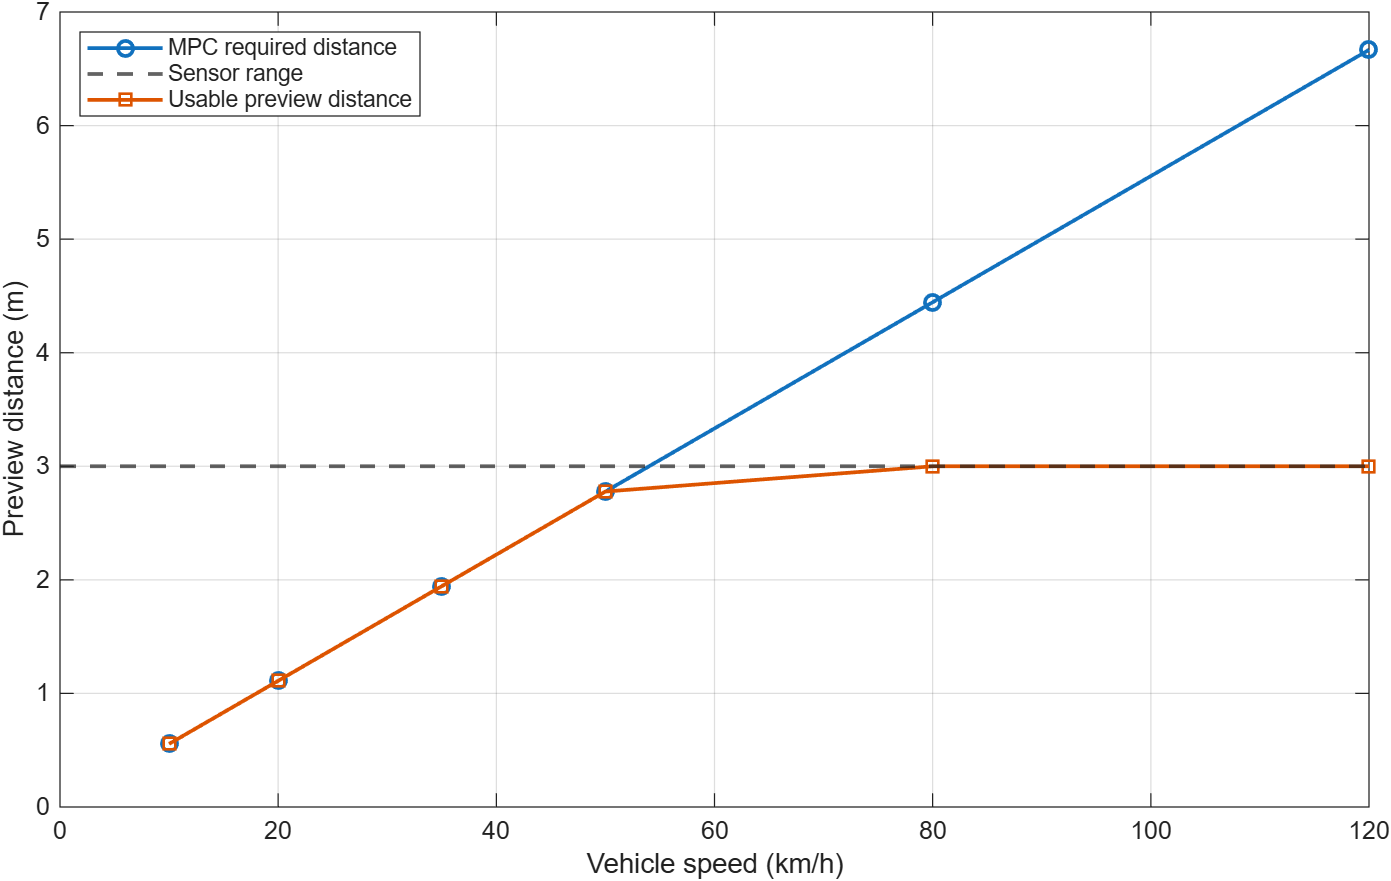
\includegraphics[width=0.82\linewidth]{speed_distance_mapping.png}
  \caption{固定 \SI{3}{m} 感知距离与不同车速下的 MPC 所需预瞄距离。$N=20$、$T_s=\SI{10}{ms}$ 时，\SI{35}{km/h} 需要 \SI{1.94}{m}，覆盖率为 100\%；\SI{80}{km/h} 时只能覆盖 67.5\% 的预测域。}
  \label{fig:speed_distance}
\end{figure}

图~\ref{fig:speed_distance} 说明，预瞄距离不应随意固定为某个时间长度。当前 \SI{3}{m} 传感器在 \SI{50}{km/h} 及以下可以覆盖 20 步预测域；在 \SI{80}{km/h} 和 \SI{120}{km/h} 时，完整预测域分别需要 \SI{4.44}{m} 和 \SI{6.67}{m}。高速工况应在增加传感器有效距离、缩短预测步数或采用随车速调度的预测域之间作选择。

\subsection{预瞄误差与鲁棒行程边界}

代码对道路高程和空间斜率分别给出盒式误差边界 $\bar e_z(\ell)$ 与 $\bar e_s(\ell)$，并允许误差随距离增大。将各步误差堆叠为 $\Delta\vect{W}$，满足
\begin{equation}
|\Delta\vect{W}|\leq \bar{\vect{W}},
\end{equation}
则道路误差对预测悬架行程的最坏影响上界为
\begin{equation}
\vect{m}_{r}=|\vect{T}_w|\,\bar{\vect{W}}\oslash\vect{s}_{\max},
\end{equation}
其中 $\vect{T}_w$ 为道路输入到行程的预测矩阵，$\vect{s}_{\max}$ 为行程上限，$\oslash$ 表示逐元素除法。在线约束据此收紧为
\begin{equation}
-\vect{1}+\vect{m}_{r}
\leq \vect{T}_{s}\vect{V}+\vect{t}(\vect{x}_0,\hat{\vect{W}})
\leq \vect{1}-\vect{m}_{r}.
\end{equation}
当前实现将单步最大收紧比例限制为 25\%，防止感知范围外的保守误差直接使 QP 无解。该处理属于约束鲁棒化，还不是带不变集反馈的完整管束 MPC。

\subsection{预测矩阵}

将预测域内的状态、控制和道路扰动分别堆叠为
\begin{equation}
\vect{X}=\begin{bmatrix}\vect{x}_1\\\vdots\\\vect{x}_N\end{bmatrix},\quad
\vect{U}=\begin{bmatrix}\vect{u}_0\\\vdots\\\vect{u}_{N-1}\end{bmatrix},\quad
\vect{W}=\begin{bmatrix}\vect{w}_0\\\vdots\\\vect{w}_{N-1}\end{bmatrix}.
\end{equation}
则
\begin{equation}
\vect{X}=\vect{S}_x\vect{x}_0+\vect{S}_u\vect{U}+\vect{S}_w\vect{W},
\end{equation}
其中
\begin{align}
\vect{S}_x&=
\begin{bmatrix}
\vect{A}_d\\ \vect{A}_d^2\\ \vdots\\ \vect{A}_d^N
\end{bmatrix},\\[2mm]
\vect{S}_u&=
\begin{bmatrix}
\vect{B}_d & \vect{0} & \cdots & \vect{0}\\
\vect{A}_d\vect{B}_d & \vect{B}_d & \cdots & \vect{0}\\
\vdots & \vdots & \ddots & \vdots\\
\vect{A}_d^{N-1}\vect{B}_d & \vect{A}_d^{N-2}\vect{B}_d & \cdots & \vect{B}_d
\end{bmatrix}.
\end{align}
$\vect{S}_w$ 与 $\vect{S}_u$ 具有相同下三角结构，只需将 $\vect{B}_d$ 替换为 $\vect{E}_d$。

堆叠输出为
\begin{equation}
\vect{Y}=\vect{Y}_x\vect{x}_0+\vect{M}_y\vect{U}+\vect{Y}_w\vect{W},
\end{equation}
其中
\begin{equation}
\vect{Y}_x=\bar{\vect{C}}_y\vect{S}_x,\quad
\vect{M}_y=\bar{\vect{C}}_y\vect{S}_u+\bar{\vect{D}}_y,\quad
\vect{Y}_w=\bar{\vect{C}}_y\vect{S}_w+\bar{\vect{F}}_y.
\end{equation}

\section{有限时域 QP-MPC}

\subsection{无量纲控制变量与差分算子}

为改善数值条件，使用轴力上限构造对角尺度矩阵 $\vect{S}_F$，并令
\begin{equation}
\vect{U}=\vect{S}_F\vect{V}.
\end{equation}
$\vect{V}$ 为无量纲决策变量。令 $\vect{D}$ 为一阶差分矩阵，则
\begin{equation}
\Delta\vect{U}=\vect{D}\vect{S}_F\vect{V}+\vect{d}(\vect{u}_{-1}).
\end{equation}
差分矩阵为
\begin{equation}
\vect{D}=\begin{bmatrix}
\vect{I} & \vect{0} & \cdots & \vect{0}\\
-\vect{I} & \vect{I} & \cdots & \vect{0}\\
\vdots & \vdots & \ddots & \vdots\\
\vect{0} & \vect{0} & -\vect{I} & \vect{I}
\end{bmatrix}.
\end{equation}

\subsection{性能指标}

有限时域代价函数为
\begin{equation}
J=\vect{Y}\trans\vect{Q}_y\vect{Y}
+\vect{V}\trans\vect{R}_u\vect{V}
+(\Delta\vect{U})\trans\vect{R}_{\Delta u}(\Delta\vect{U}).
\end{equation}

输出权重向量及对应物理尺度为
\begin{align}
\vect{q}_y&=\begin{bmatrix}5.00&2.00&0.020&0.020&0.010&0.010\end{bmatrix}\trans,\\
\vect{s}_y&=\begin{bmatrix}1.0&0.75&0.040&0.050&0.025&0.025\end{bmatrix}\trans,\\
\vect{Q}_y&=\vect{I}_N\otimes\diag\!\left(\frac{q_{y,i}}{s_{y,i}^2}\right).
\end{align}
当前 $\vect{R}_u=0.40\vect{I}$，$\vect{R}_{\Delta u}=0.20\vect{I}$。这些权重来自 CarSim 在环的小规模筛选。旧配置对悬架行程的归一化惩罚过大，虽然能够压缩行程，却会恶化车身和俯仰加速度；本次重新整定后把舒适性指标放在首位，同时保留行程和轮胎挠度代价。

令
\begin{equation}
\vect{c}=\vect{Y}_x\vect{x}_0+\vect{Y}_w\vect{W},\qquad
\vect{D}_s=\diag(\Delta\vect{u}_{\max}^{-1})\vect{D}\vect{S}_F,
\end{equation}
则代价可凝聚为标准二次规划
\begin{equation}
\min_{\vect{V}}\;\frac{1}{2}\vect{V}\trans\vect{H}\vect{V}+\vect{f}\trans\vect{V},
\end{equation}
其中
\begin{align}
\vect{H}=2\Big[&
(\vect{M}_y\vect{S}_F)\trans\vect{Q}_y(\vect{M}_y\vect{S}_F)
+\vect{R}_u+\vect{D}_s\trans\vect{R}_{\Delta u}\vect{D}_s\Big],\\
\vect{f}=2\Big[&
(\vect{M}_y\vect{S}_F)\trans\vect{Q}_y\vect{c}
+\vect{D}_s\trans\vect{R}_{\Delta u}\vect{d}_s\Big].
\end{align}

\subsection{在线硬约束}

当前实现的在线硬约束为
\begin{align}
-\vect{1}&\le \vect{V}\le \vect{1},\\
-\vect{1}&\le \vect{D}_s\vect{V}+\vect{d}_s\le \vect{1},\\
-\vect{1}&\le \vect{T}_s\vect{V}+\vect{t}(\vect{x}_0,\vect{W})\le \vect{1},
\end{align}
即
\begin{equation}
|F_f|,|F_r|\le \SI{2000}{N},\qquad
|\Delta F_f|,|\Delta F_r|\le \SI{1000}{N/sample}.
\end{equation}
第三组约束对应前、后悬架预测行程，边界均为 $\pm\SI{0.080}{m}$。$\vect{T}_s$ 为归一化行程预测矩阵，$\vect{t}(\vect{x}_0,\vect{W})$ 汇总当前状态和道路预瞄产生的仿射项。

因此 QP 约束矩阵为
\begin{equation}
\vect{A}_{\text{con}}=
\begin{bmatrix}\vect{I}\\\vect{D}_s\\\vect{T}_s\end{bmatrix},
\qquad
\vect{l}\le\vect{A}_{\text{con}}\vect{V}\le\vect{u}.
\end{equation}

\begin{notebox}{行程约束的可行性}
悬架行程已经进入在线约束，但当前仍采用无松弛变量的硬边界。行程上限曾设为前 \SI{45}{mm}、后 \SI{55}{mm}，而 CarSim 的被动 C 级路面工况前悬行程已达到 \SI{67.3}{mm}，使 QP 在有限作动力下不可行。现将边界统一为 \SI{80}{mm}，与该悬架模型的工作区间相符。后续仍应增加松弛变量和不可行降级逻辑，以避免极端路面下的数值残差。
\end{notebox}

\subsection{ADMM 在线求解}

当前实现没有调用 Optimization Toolbox 或 OSQP 库。\path{qp_admm.m} 使用基于算子分裂的 ADMM 迭代求解
$\vect{l}\le\vect{A}_{\text{con}}\vect{V}\le\vect{u}$，迭代形式与 OSQP 的基本分裂框架相近。第 $j$ 次迭代为
\begin{align}
\vect{V}^{j+1}={}&
\left(\vect{H}+\sigma\vect{I}+\rho\vect{A}_{\text{con}}\trans\vect{A}_{\text{con}}\right)^{-1}
\left[-\vect{f}+\sigma\vect{V}^{j}
+\rho\vect{A}_{\text{con}}\trans(\vect{z}^{j}-\vect{y}^{j})\right],\\
\vect{z}^{j+1}={}&
\Pi_{[\vect{l},\vect{u}]}
\left(\vect{A}_{\text{con}}\vect{V}^{j+1}+\vect{y}^{j}\right),\\
\vect{y}^{j+1}={}&
\vect{y}^{j}+\vect{A}_{\text{con}}\vect{V}^{j+1}-\vect{z}^{j+1}.
\end{align}
其中 $\Pi_{[\vect{l},\vect{u}]}$ 表示逐元素区间投影。当前参数为
$\rho=1$、$\sigma=10^{-7}$、最大迭代次数 800，绝对与相对容差均为 $2\times10^{-4}$。求解器使用上一时刻结果热启动，并只下发最优序列的首个控制量。

\section{线性被动悬架、四角力分配与安全门控}

CarSim 的导入顺序为 $L1,L2,R1,R2$。线性被动阻尼力按四个减振器压缩速度计算：
\begin{equation}
\vect{F}_{\text{base}}=c_b
\begin{bmatrix}
\mathrm{CmpRD}_{L1}&\mathrm{CmpRD}_{L2}&\mathrm{CmpRD}_{R1}&\mathrm{CmpRD}_{R2}
\end{bmatrix}\trans,
\qquad c_b=\SI{3}{N/(mm/s)}.
\end{equation}
CarSim 将 $\mathrm{Fd}$ 定义为压缩方向阻尼力，将 $\mathrm{CmpRD}$ 定义为减振器压缩速度。因此四角阻尼的耗散功率为
\begin{equation}
P_{\text{loss}}
=\frac{1}{1000}\sum_i F_{\text{base},i}\,\mathrm{CmpRD}_i
=\frac{c_b}{1000}\sum_i \mathrm{CmpRD}_i^2\geq 0,
\end{equation}
式中因速度单位为 \si{mm/s}，故除以 1000 后功率单位为瓦。只要 $c_b>0$，阻尼元件就只耗散能量，不会向车身主动注入能量。因此该基线属于线性被动悬架等效实验，只是用固定线性阻尼律替换了 CarSim 原生非线性减振器曲线；弹簧力和轮胎力仍由 CarSim 整车模型内部计算。

被动基线取 $\alpha=0$，控制器跳过 QP 求解，只保留弹簧力和线性阻尼力。主动工况取 $\alpha=1$，前、后轴力分别分配到左右车轮：
\begin{equation}
\begin{bmatrix}
F_{L1}\\F_{L2}\\F_{R1}\\F_{R2}
\end{bmatrix}
=\vect{F}_{\text{base}}
+\frac{\alpha}{2}
\begin{bmatrix}
F_f\\F_r\\F_f\\F_r
\end{bmatrix}.
\end{equation}
最终下发值为
\begin{equation}
\vect{F}_{\text{cmd}}
=\sat_{[-5000,5000]}\!\left(\vect{F}_{\text{base}}+\vect{F}_{\text{MPC}}\right).
\end{equation}

若输入维度异常或出现非有限值，控制器返回零主动命令，并保留线性被动阻尼力。QP 首个轴力在下发前还要经过力限幅和变化率投影；四角总力随后限制在 $\pm\SI{5000}{N}$。由于预测模型的输入矩阵含有 $\alpha\gamma_f$ 和 $\alpha\gamma_r$，优化器预测的广义轴力与实际部署链保持一致。

\subsection{持续主动力与 CDC 工程约束}

理想主动力结果用于检验 MPC 的控制上限。为模拟量产执行链，代码还提供两种部署模式。持续主动力模式每 \SI{50}{ms} 才允许更新一次目标，目标量化到 \SI{100}{N}，模式至少保持 \SI{100}{ms}，执行器用时间常数 $\tau_a=\SI{30}{ms}$ 的一阶环节逼近目标：
\begin{equation}
F_{a,k+1}=F_{a,k}+\left(1-\exp(-T_s/\tau_a)\right)
\left(F_{a,k}^{\star}-F_{a,k}\right).
\end{equation}
预测域内前 10 个控制步还加入相等约束，以避免优化器假设这段保持时间内可以连续改写命令。

CDC 模式不再直接施加任意作动力。设单轴两角平均减振器速度为 $v_{d,j}$，主动 MPC 希望增加的轴力为 $F_j^{\star}$，则先计算等效目标阻尼
\begin{equation}
c_{j}^{\star}=c_b+\frac{F_j^{\star}}{2v_{d,j}},
\qquad |v_{d,j}|\geq \SI{5}{mm/s},
\end{equation}
再投影到 $\{1.5,2.25,3.0,4.0,5.0\}\,\si{N/(mm/s)}$ 五档阻尼。档位同样满足 \SI{50}{ms} 判定周期、\SI{100}{ms} 最小保持时间和 \SI{30}{ms} 响应时间。该映射保证阻尼力与减振器速度同号，但不能实现任意符号的主动轴力，因此必须与理想主动悬架结果分开评价。

\section{仿真结果与讨论}

\subsection{离线 QP 数值检查}

离线检查确认输入矩阵中的等效系数为 $[0.65144,\,0.79700]\trans$，对应前、后悬架运动比；角点阻尼换算后的前、后轴阻尼为 \SI{2546.2}{N.s/m} 和 \SI{3811.3}{N.s/m}。代表性 QP 在 140 次迭代后收敛，最大约束残差为 $3.89\times10^{-4}$。联合仿真中轴力命令上限为 \SI{2000}{N}，单步轴力增量上限为 \SI{1000}{N}，下发前仍执行一次力和变化率投影。

\subsection{线性被动悬架与预瞄 QP-MPC 对比}

\begin{table}[H]
\centering
\caption{\SI{35}{km/h} C 级道路 \SI{20}{s} 单次工况复核}
\begin{tabularx}{\linewidth}{X l S[table-format=4.5] S[table-format=4.5] S[table-format=2.3]}
\toprule
指标 & 单位 & {被动基线} & {被动基线 + MPC} & {变化(\%)}\\
\midrule
车身加速度 RMS & \si{m/s^2} & 2.12820 & 1.58320 & 25.608\\
俯仰角加速度 RMS & \si{rad/s^2} & 0.04556 & 0.03102 & 31.918\\
前悬架峰值行程 & \si{m} & 0.06740 & 0.05622 & 16.590\\
后悬架峰值行程 & \si{m} & 0.05265 & 0.03945 & 25.063\\
下发角点力峰值 & \si{N} & 3942.02 & 3819.40 & 3.110\\
QP 原始解最大约束超限 & -- & 0 & 0.00993 & {--}\\
QP 收敛比例 & \si{\percent} & 100.000 & 99.050 & {--}\\
\bottomrule
\end{tabularx}
\end{table}

两组实验使用同一车辆、道路、车速和线性阻尼律，差别只有 MPC 主动力。车身和俯仰角加速度 RMS 分别降低 \SI{25.61}{\percent} 和 \SI{31.92}{\percent}，前、后悬架峰值行程也同步下降。\SI{1}{ms} 结果与原 \SI{0.5}{ms} 参考值的加速度 RMS 相差约 1\%，说明减小积分次数没有改变主要结论。QP 收敛比例和原始解约束超限属于求解器诊断量，不是车辆性能指标。

\subsection{坑包、B 级和 C 级道路对比}

三类道路均以 \SI{35}{km/h} 运行 \SI{12}{s}，统计时忽略前 \SI{0.5}{s} 初始化段。坑包道路包含一个 \SI{50}{mm} 凸包和一个 \SI{50}{mm} 凹坑；B、C 级道路直接使用当前 CarSim 数据库的空间高程表。表中正值表示 MPC 低于被动基线，负值表示指标增加。

\begin{table}[H]
\centering
\caption{三类道路主要指标相对被动悬架的变化率}
{\small
\begin{tabular}{l S[table-format=2.2] S[table-format=2.2] S[table-format=2.2] S[table-format=-2.2]}
\toprule
道路 & {车身加速度 RMS} & {俯仰加速度 RMS} & {最大行程$^\ast$} & {轮胎动载 RMS}\\
 & {(\%)} & {(\%)} & {(\%)} & {(\%)}\\
\midrule
坑包道路 & 15.29 & 13.43 & 2.90 & -6.49\\
B 级道路 & 32.87 & 40.90 & 24.75 & -25.20\\
C 级道路 & 25.13 & 31.12 & 16.59 & -1.70\\
\bottomrule
\multicolumn{5}{l}{\footnotesize $^\ast$取前、后悬架改善率中较小者。}
\end{tabular}}
\end{table}

\begin{figure}[H]
  \centering
  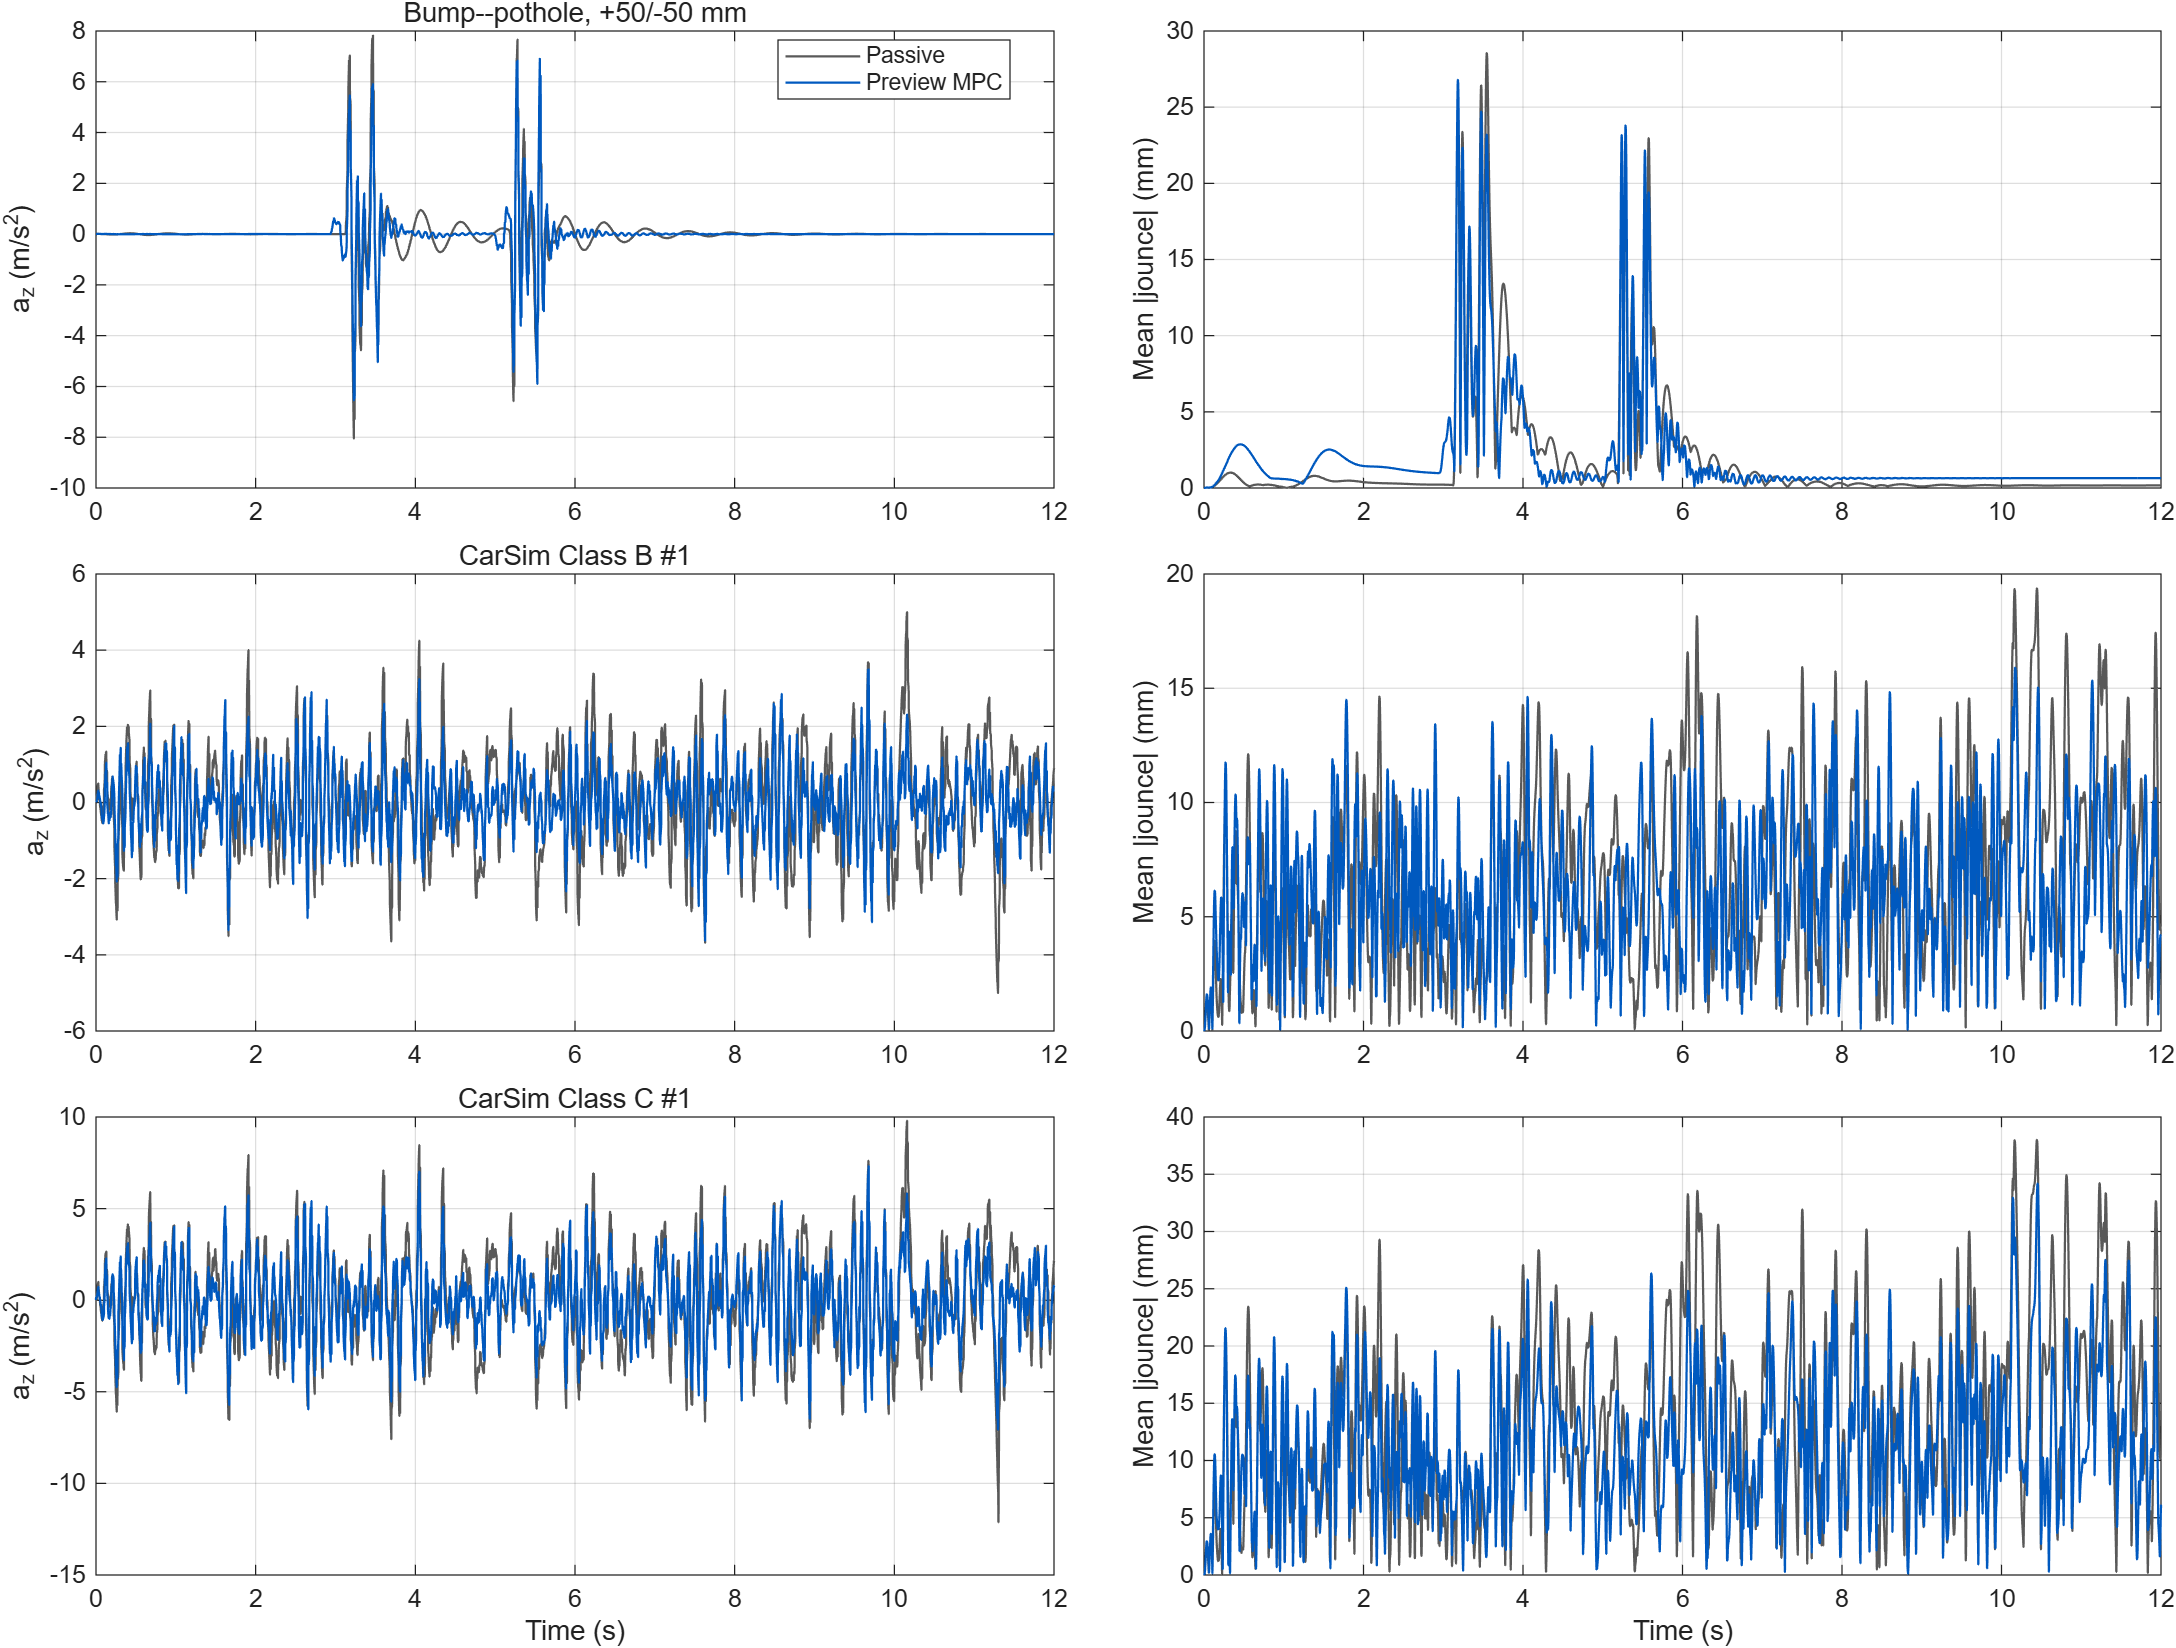
\includegraphics[width=0.98\linewidth]{road_suite_response.png}
  \caption{坑包、B 级和 C 级道路下的车身垂向加速度与平均悬架行程。灰线为线性被动悬架，蓝线为道路预瞄 QP-MPC。}
  \label{fig:road_suite_response}
\end{figure}

图~\ref{fig:road_suite_response} 与表中结果一致：MPC 在三类道路上均降低车身和俯仰响应，并压缩悬架行程。代价是轮胎动载 RMS 上升，其中 B 级路面增幅为 \SI{25.20}{\percent}。坑包工况的角点总力还达到 \SI{5000}{N} 饱和边界，因此其峰值结论应谨慎解释。现阶段只能说控制器改善了舒适性和姿态响应，不能据此声称综合性能全面优于被动悬架。后续需要提高轮胎挠度权重，或将轮胎动载写成显式软约束，并重新检查舒适性与接地性的 Pareto 权衡。

\subsection{不同车速下的空间等距对照}

车速实验取 \SI{35}{km/h}、\SI{60}{km/h} 和 \SI{80}{km/h}，每个车速均重复坑包、B 级和 C 级道路的被动/MPC 对照。统计区间统一为前轮道路坐标 \SI{10}{m}--\SI{110}{m}，仿真终止时间随车速调整。这样三组车速经过相同的道路样本，也不会在高速车辆驶出道路高程表后混入额外的平路响应。CarSim 记录的平均车速分别为 \SI{34.94}{km/h}、\SI{59.93}{km/h} 和 \SI{79.93}{km/h}，与目标值一致。

\begin{table}[H]
\centering
\caption{不同车速下 MPC 相对线性被动悬架的变化率。正值表示指标降低，负值表示指标增加；各行均按前轮 \SI{10}{m}--\SI{110}{m} 的道路区间统计。}
\label{tab:speed_suite}
{\small
\begin{tabular}{l c S[table-format=2.2] S[table-format=2.2] S[table-format=3.2] S[table-format=-2.2]}
\toprule
道路 & {车速} & {车身加速度 RMS} & {俯仰加速度 RMS} & {最小预瞄覆盖率} & {轮胎动载 RMS}\\
 & {(km/h)} & {(\%)} & {(\%)} & {(\%)} & {(\%)}\\
\midrule
坑包 & 35 & 15.29 & 13.43 & 100.00 & -6.49\\
坑包 & 60 & 16.43 & 6.59 & 89.98 & -11.88\\
坑包 & 80 & 15.35 & 13.63 & 67.50 & -7.82\\
\addlinespace
B 级 & 35 & 33.24 & 41.22 & 100.00 & -24.73\\
B 级 & 60 & 38.14 & 26.30 & 89.90 & -14.05\\
B 级 & 80 & 36.14 & 24.02 & 67.47 & -11.81\\
\addlinespace
C 级 & 35 & 25.21 & 31.45 & 100.00 & -1.44\\
C 级 & 60 & 30.39 & 18.57 & 89.77 & 2.52\\
C 级 & 80 & 24.91 & 13.16 & 67.42 & 0.93\\
\bottomrule
\end{tabular}}
\end{table}

\begin{figure}[H]
  \centering
  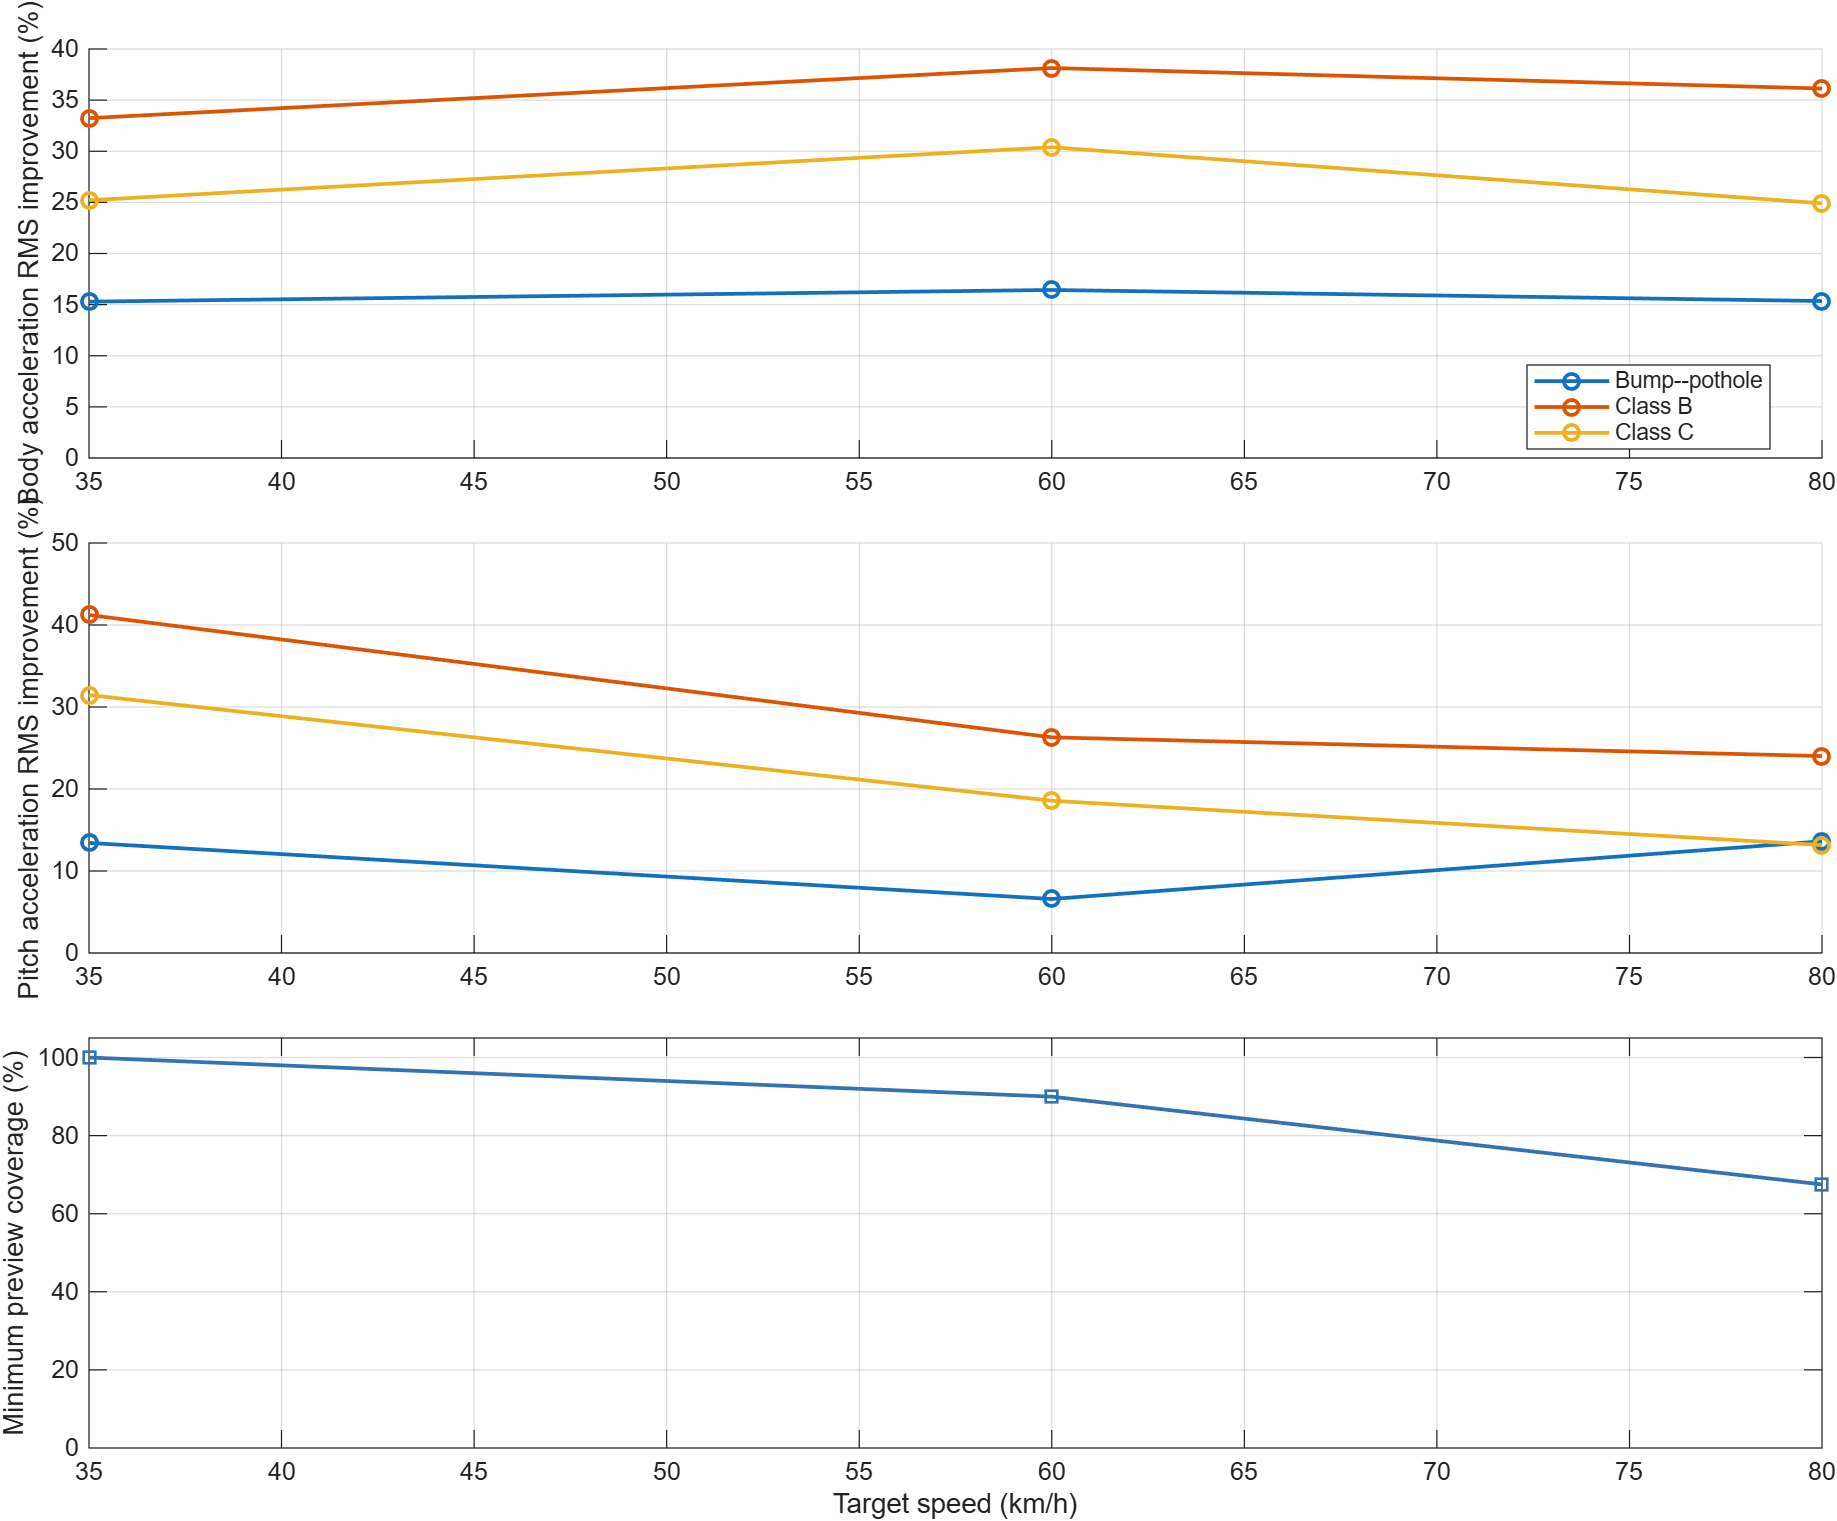
\includegraphics[width=0.94\linewidth]{speed_suite_summary.png}
  \caption{不同车速下的车身、俯仰角加速度 RMS 改善率及固定 \SI{3}{m} 传感器的最小预瞄覆盖率。预测步数保持为 $N=20$，控制周期保持为 \SI{10}{ms}。}
  \label{fig:speed_suite}
\end{figure}

表~\ref{tab:speed_suite} 和图~\ref{fig:speed_suite} 给出两个结论。第一，九组工况的车身和俯仰角加速度 RMS 均低于被动基线，车身改善率为 \SI{15.29}{\percent}--\SI{38.14}{\percent}；车身舒适性收益在本次车速范围内没有消失。第二，高速下的控制余量正在收窄。20 步预测域所需距离由 \SI{35}{km/h} 时的 \SI{1.94}{m} 增至 \SI{60}{km/h} 时的 \SI{3.33}{m} 和 \SI{80}{km/h} 时的 \SI{4.44}{m}，固定 \SI{3}{m} 传感器只能覆盖后两者的约 \SI{89.8}{\percent} 和 \SI{67.4}{\percent}。B、C 级道路的俯仰改善率也随车速升高而下降。

该趋势不能只归因于预瞄截断，因为车速同时改变了道路激励的时间频率以及降阶模型与 CarSim 的动态失配。另一个需要保留的负面结果是：坑包工况在 \SI{60}{km/h} 时前、后最大行程分别增加 \SI{1.67}{\percent} 和 \SI{9.66}{\percent}，在 \SI{80}{km/h} 时分别增加 \SI{7.80}{\percent} 和 \SI{8.73}{\percent}；多数工况的轮胎动载也高于被动基线。因此，当前控制器可以支持多车速下的舒适性结论，但还不能采用一套固定权重宣称全车速综合性能改善。下一步应把传感器有效距离、预测步数和权重按车速联合调度，并用更密集的车速网格复核。

\subsection{感知误差与短预瞄距离}

为避免把控制器直接接到“完全准确的道路真值”，C 级道路实验在固定空间坐标上加入相关噪声和偏置。表~\ref{tab:robustness} 中的鲁棒收紧比例表示预测行程边界被预留的最大份额。

\begin{table}[H]
\centering
\caption{C 级道路空间感知误差与鲁棒约束实验}
\label{tab:robustness}
{\small
\begin{tabularx}{\linewidth}{X S[table-format=2.2] S[table-format=2.2] S[table-format=3.2] S[table-format=2.2]}
\toprule
工况 & {车身 RMS 改善} & {俯仰 RMS 改善} & {最小覆盖率} & {最大收紧比例}\\
 & {(\%)} & {(\%)} & {(\%)} & {(\%)}\\
\midrule
无感知误差，开启收紧 & 25.13 & 31.12 & 100.00 & 14.49\\
\SI{2}{mm} 噪声 + \SI{1}{mm} 偏置，开启收紧 & 24.82 & 30.92 & 100.00 & 14.49\\
相同误差，关闭收紧 & 24.82 & 30.92 & 100.00 & 0.00\\
\SI{5}{mm} 噪声 + \SI{2}{mm} 偏置，\SI{1.5}{m} 范围 & 23.47 & 29.24 & 76.68 & 25.00\\
\bottomrule
\end{tabularx}}
\end{table}

\begin{figure}[H]
  \centering
  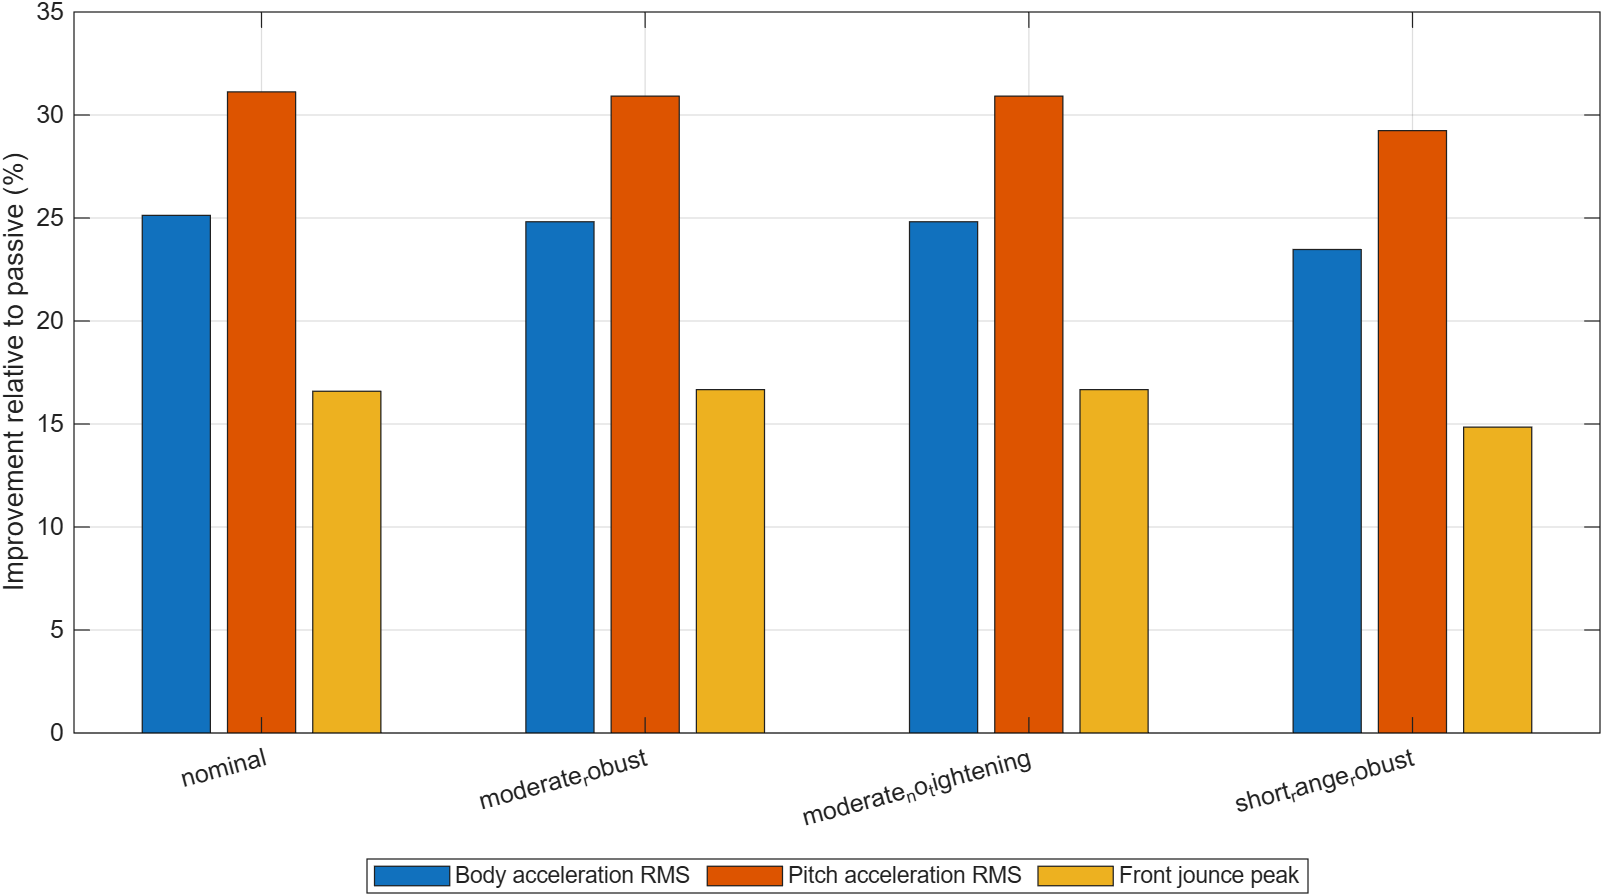
\includegraphics[width=0.88\linewidth]{robustness_summary.png}
  \caption{C 级道路不同空间预瞄误差下，相对线性被动悬架的改善率。误差固定在道路坐标上，正值表示指标下降。}
  \label{fig:robustness}
\end{figure}

中等误差只使车身 RMS 改善率下降 0.31 个百分点；更大误差和较短感知距离下仍保留 \SI{23.47}{\percent} 的改善。该结果表明当前闭环对这组误差不敏感，但不能把它归因于约束收紧：开启与关闭收紧的车辆响应相同，说明 \SI{80}{mm} 行程边界在该工况下没有成为活跃约束。开启收紧时最大行程裕量为 14.49\%，短距离工况达到设定上限 25\%。它提供了安全余量，却尚未带来可测的性能差异。更严格的鲁棒性结论还需要多随机种子、感知延迟、丢帧和参数摄动试验。

\subsection{执行持续时间与 CDC 映射}

表~\ref{tab:deployment} 比较理想主动力、持续主动力和五档 CDC 部署。三组实验使用相同 QP 权重；持续主动力与 CDC 均采用 \SI{50}{ms} 判定周期、\SI{100}{ms} 最小保持时间和 \SI{30}{ms} 一阶响应。

\begin{table}[H]
\centering
\caption{不同执行链相对线性被动悬架的 RMS 改善率}
\label{tab:deployment}
{\small
\begin{tabular}{l l S[table-format=-2.2] S[table-format=-2.2]}
\toprule
部署方式 & 道路 & {车身加速度 RMS (\%)} & {俯仰加速度 RMS (\%)}\\
\midrule
理想主动力 & 坑包 & 15.29 & 13.43\\
理想主动力 & B 级 & 32.87 & 40.90\\
理想主动力 & C 级 & 25.13 & 31.12\\
持续主动力 & 坑包 & 2.86 & 5.04\\
持续主动力 & B 级 & 8.91 & 13.41\\
持续主动力 & C 级 & 4.86 & 7.15\\
五档 CDC & 坑包 & -1.34 & -4.67\\
五档 CDC & B 级 & -4.29 & -1.35\\
五档 CDC & C 级 & -3.26 & -0.50\\
\bottomrule
\end{tabular}}
\end{table}

更新变慢后，持续主动力版本仍能改善 B、C 级道路的 RMS 指标，但效果明显低于理想执行链。五档 CDC 的 RMS 指标则普遍略差于固定 \SI{3}{N/(mm/s)} 被动基线。这一结果并不支持“主动 MPC 命令经限幅即可用于 CDC”的假设：主动 QP 可以要求任意方向的轴力，CDC 只能沿当前减振器速度方向耗散能量，\SI{100}{ms} 保持还会延长不合适档位的作用时间。后续 CDC 控制器应直接以阻尼系数或离散档位为决策变量，并把半主动可实现约束写入预测模型。

\subsection{MPC 设计复核}

完成参数和接口修正后，又在 CarSim 中对 $N=10,15,20,30$ 进行了同工况扫描。结果如下：

\begin{table}[H]
\centering
\caption{CarSim 在环的预测时域扫描}
\begin{tabular}{c c S[table-format=2.2] S[table-format=2.2] S[table-format=1.4]}
\toprule
$N$ & 预瞄时间 / s & {车身加速度改善 / \%} & {俯仰加速度改善 / \%} & {QP 收敛率}\\
\midrule
10 & 0.10 & 19.10 & 21.41 & 0.9917\\
15 & 0.15 & 23.88 & 29.15 & 0.9759\\
20 & 0.20 & 25.09 & 30.82 & 0.9850\\
30 & 0.30 & 25.80 & 31.67 & 0.9817\\
\bottomrule
\end{tabular}
\end{table}

最终配置下，四个预测域都能降低车身和俯仰响应。$N$ 从 20 增加到 30 时，车身和俯仰 RMS 改善率只增加 0.72 和 0.85 个百分点，而主动工况的仿真实时比由约 0.27 增加到 0.76。$N=20$ 因此是效果与计算量之间的折中，并不存在“当前 20 步预瞄过长”的证据。先前控制效果差的主要原因不是预测域，而是以下三项接口错误和权重失配：
\begin{enumerate}
  \item 预测模型曾将被动阻尼高估约 3.8 倍；现已按 \SI{3}{N/(mm/s)} 角点阻尼重新折算。
  \item QP 曾按完整轴力预测，而执行端只部署 $\alpha=0.10$；现取 $\alpha=1$，并把悬架运动比和部署比例直接写入 $\vect{B}$。
  \item CarSim 的 \texttt{Pitch/AVy} 与半车模型的车头上仰正方向相反。未换算时，俯仰反馈会放大响应；乘以 $-1$ 后，最终 \SI{20}{s} 工况的车身与俯仰加速度 RMS 分别改善 \SI{25.61}{\percent} 和 \SI{31.92}{\percent}。
\end{enumerate}

此外，旧权重过度压缩悬架行程。CarSim 在环筛选后提高了车身和俯仰加速度权重，并降低行程、轮胎挠度以及控制力权重。修正后的三类道路结果均为正向，但轮胎动载上升，说明当前权重仍是偏舒适性的折中，不是最终标定。

\section{CarSim 动画与视频导出}

CarSim 2020 的 VS Visualizer 在 Windows 下可以将全部或部分动画直接导出为 AVI，当前仿真生成的 \texttt{LastRun.vs} 和 \texttt{LastRun.vsb} 可用于回放和导出。

\begin{enumerate}
  \item 在 CarSim Run Control 页面打开 \texttt{Video}，或在 VS Visualizer 中打开 \texttt{LastRun.vs}；
  \item 调整相机角度、缩放和动画窗口尺寸，窗口尺寸即视频导出分辨率；
  \item 选择 \texttt{File -> Export Video}，或在动画区域右键选择 \texttt{Export Video}；
  \item 指定 AVI 路径；勾选 \texttt{Set Video Time} 可设置起止时间，不勾选则导出完整动画；
  \item 在 \texttt{Video Compression} 对话框中选择系统已安装的编码器并开始导出。
\end{enumerate}

VS Visualizer 导出的 AVI 不含音频。若需要论文答辩或网页常用的 MP4，可先导出无损或高质量 AVI，再使用 \texttt{ffmpeg} 转码为 H.264 MP4。本节依据本机 CarSim 2020 官方手册《VS Visualizer Reference Manual》第 26--27 页。

\section{尚存问题与后续安排}

\begin{longtable}{>{\raggedright\arraybackslash}p{13mm}>{\raggedright\arraybackslash}p{0.49\linewidth}>{\raggedright\arraybackslash}p{0.32\linewidth}}
\caption{当前缺陷及处理顺序}\label{tab:next_steps}\\
\toprule
优先级 & 当前缺陷 & 处理方式\\
\midrule
\endfirsthead
\toprule
优先级 & 当前缺陷 & 处理方式\\
\midrule
\endhead
P0 & CarSim 导入和导出配置重复，当前依赖 77 路兼容映射 & 清理重复配置并固定 39 路完整映射\\
P0 & 多车速实验的最低 QP 收敛比例为 \SI{94.44}{\percent}（\SI{80}{km/h} C 级道路），且没有单步求解时间统计 & 加入行程松弛变量，检查 ADMM 停止条件，并记录平均、95 分位和最坏求解时间\\
P0 & 半车其余参数由整车参数折算，尚未用 CarSim 数据辨识 & 用扫频、随机路和脉冲路数据辨识并留出独立验证工况\\
P0 & 主动力 MPC 直接映射到五档 CDC 后，三类道路 RMS 指标均未改善 & 以阻尼档位为决策变量，显式加入半主动可实现域和最小保持时间，再单独整定 CDC-MPC\\
P1 & 状态由左右平均和差分重构，对噪声较敏感 & 增加 Kalman 滤波或移动窗状态估计\\
P1 & 轮胎动载尚无显式约束，B 级路面 RMS 增加 \SI{25.20}{\percent} & 增大轮胎挠度权重，增加软约束并绘制舒适性--接地性 Pareto 曲线\\
P1 & 目前只有三个离散车速，且每个车速--道路组合仍是单次运行 & 增加车速网格、感知延迟、丢帧、误差种子和车辆参数摄动的重复试验\\
P2 & 半车控制器不能处理侧倾和左右不对称道路 & 升级为含侧倾和四轮独立作动力的整车 MPC\\
\bottomrule
\end{longtable}

在形成论文结论前，至少需要报告车身垂向加速度 RMS/PSD、俯仰与侧倾角加速度、悬架动行程、轮胎动载荷、控制能耗、约束触发比例和求解时间。对比组应包含 CarSim 原生非线性被动悬架、当前线性被动悬架等效基线、Skyhook、无预瞄 MPC 和预瞄 MPC，并明确参数选择依据和重复次数。

\section{复现实验入口}

\begin{enumerate}
  \item 在 MATLAB 中进入 \texttt{carsim\_mpc\_quick}，加入 \texttt{src} 与 \texttt{tests} 路径；
  \item 运行 \texttt{validate\_quick\_mpc\_offline()} 检查 QP 数值、收敛和约束；
  \item 首次运行或接口变化后执行 \texttt{build\_carsim\_mpc\_model()}；
  \item 运行 \texttt{tune\_quick\_mpc\_carsim()} 核查权重和 CarSim 力接口极性；
  \item 运行 \texttt{run\_carsim\_mpc\_horizon\_sweep()} 比较 $N=10,15,20,30$；
  \item 运行 \texttt{run\_carsim\_mpc\_demo()}，依次执行线性被动悬架基线与 $\alpha=1$ 的主动工况；
  \item 运行 \texttt{run\_carsim\_mpc\_road\_suite()} 完成坑包、B 级和 C 级道路对照；
  \item 运行 \texttt{run\_carsim\_mpc\_speed\_suite([35 60 80])}，按统一道路坐标区间完成三车速对照；
  \item 分别以 \texttt{'persistent\_force'} 和 \texttt{'cdc'} 调用多路面脚本，检查更新周期、保持时间和阻尼档位影响；
  \item 运行 \texttt{run\_carsim\_mpc\_robustness\_suite()}，比较空间噪声、偏置、短感知距离与约束收紧；
  \item 检查主结果文件和各 \texttt{road\_suite} 目录：\\
    \path{results/carsim_mpc_quick/metrics.csv}，\\
    \path{results/carsim_mpc_quick/carsim_mpc_run.mat}；
  \item 检查鲁棒性汇总和各工况的 CarSim 回放文件：\\
    \path{robustness_suite/robustness_metrics.csv}，\\
    \path{LastRun.vs/.vsb}。
  \item 检查多车速汇总：\\
    \path{speed_suite/speed_suite_metrics.csv}，\\
    \path{speed_suite/speed_suite_summary.png}。
\end{enumerate}

\begin{table}[H]
\centering
\caption{关键实现文件}
{\small
\begin{tabularx}{\linewidth}{p{27mm}Y Y}
\toprule
类型 & 文件 & 作用\\
\midrule
控制器配置 & \path{carsim_mpc_quick/quick_mpc_config.m} & 车辆、预测域、约束、权重和 ADMM 参数\\
半车模型 & \path{src/half_car_linear_model.m} & 连续动力学、精确离散化与性能输出\\
预测矩阵 & \path{src/build_quick_mpc_data.m} & 预测矩阵、凝聚 Hessian 和道路表\\
空间传感器 & \path{src/build_spatial_road_sensor.m} & 固定距离栅格、相关噪声和偏置\\
距离域映射 & \path{src/carsim_road_preview.m} & 由车速把空间预瞄映射到预测时域\\
QP 求解 & \path{src/preview_qp_solve.m} & 在线线性项、约束边界和首控制量\\
ADMM & \path{src/qp_admm.m} & 工具箱无关的凸 QP 迭代求解\\
联合仿真 & \path{run_carsim_mpc_demo.m} & 线性被动/主动工况运行与指标输出\\
多路面对照 & \path{run_carsim_mpc_road_suite.m} & 坑包、B 级和 C 级道路实验与绘图\\
多车速对照 & \path{run_carsim_mpc_speed_suite.m} & 三类道路在 \SI{35}{km/h}、\SI{60}{km/h} 和 \SI{80}{km/h} 下的空间等距评价\\
鲁棒性实验 & \path{run_carsim_mpc_robustness_suite.m} & 感知误差、短距离与约束收紧对照\\
\bottomrule
\end{tabularx}}
\end{table}

\section{结论}

本阶段完成了 CarSim--Simulink 接口、距离域道路感知、在线凸 QP 和四角力回写的闭环验证。控制器按 \SI{10}{ms} 周期调度，CarSim 以同步的 \SI{1}{ms} 步长积分。按前轮 \SI{10}{m}--\SI{110}{m} 的相同道路区间比较 \SI{35}{km/h}、\SI{60}{km/h} 和 \SI{80}{km/h} 后，坑包、B 级和 C 级道路的九组工况均降低了车身与俯仰角加速度 RMS，改善率分别为 \SI{15.29}{\percent}--\SI{38.14}{\percent} 和 \SI{6.59}{\percent}--\SI{41.22}{\percent}。不过，\SI{80}{km/h} 所需预瞄距离达到 \SI{4.44}{m}，固定 \SI{3}{m} 感知范围只覆盖约 \SI{67.4}{\percent}；高速坑包工况的悬架行程也有所增加。加入毫米级空间感知误差后，C 级道路仍保留约 \SI{24.82}{\percent} 的车身 RMS 改善，但多数工况的轮胎动载上升，五档 CDC 映射也没有改善 RMS 指标。当前成果可以支持“理想主动力半车预瞄 MPC 在三个离散车速下形成有效舒适性闭环”的结论，不能据此声称全车速综合性能或 CDC 控制已经完成。下一阶段应优先实现车速相关的预瞄域与权重调度，把半主动可实现域、保持时间和阻尼响应直接纳入预测模型，并增加多误差种子和参数摄动的统计试验；整车四角 MPC 则用于进一步处理侧倾和左右不对称道路。

\end{document}
